The particle physics landscape has been profoundly influenced by the discovery of a Higgs boson with a mass around 125\,GeV at the LHC~\cite{CMS:2012qbp,ATLAS:2012yve}.
The long-predicted matrix of particles and interactions of the Standard Model (SM) is now complete, and this consistent and predictive theory has so far been successful at  describing all phenomena accessible to collider experiments.
After almost 15 years of LHC operation, the remarkable precision measurements and the many exploratory searches have demonstrated its validity and excluded signs of new physics across an order of magnitude of energies around the TeV scale.
This notwithstanding, several fundamental experimental facts remain unexplained in the current framework, such as the abundance of matter over antimatter, the evidence for dark matter, or the non-zero neutrino masses, and many theoretical issues definitively also require physics beyond the present Standard Model (BSM), altogether calling for intensified collider exploration. For the first time since the Fermi theory, however, the field of possible explanations to these unanswered questions provides little guidance for what form this exploration may take.

The confirmation by the LHC of the SM predictions up to the TeV range requires a different approach to addressing these open questions. 
Solutions could exist at even higher energy, at the price of either an \emph{unnatural} value of the weak scale or an ingenious but still elusive structure. 
Instead, radically new physics scenarios have recently been devised, which  often include light and feebly coupled structures~\cite{Graham:2015cka, Espinosa:2015eda, Arkani-Hamed:2020yna}.
Neither the mass scale (from meV to ZeV) of this new physics nor the intensity of the couplings to the SM (from 1 to $10^{-12}$ or less) are known, thus calling for a new, broad, and powerful tool of exploration. 
To experimentally push the limits of the unknown as far as possible with a real chance of discovery, this tool must be able to address the following goals in the broadest and deepest possible way.

\begin{itemize}
    \item Map the properties of the Higgs and electroweak (EW) gauge bosons, pinning down their interactions with accuracies order(s) of magnitude better than today, and acquiring
    sensitivity to, e.g., the processes that led to the formation of today's Higgs vacuum field during the time span between $10^{-12}$ and $10^{-10}$\,s after the Big Bang.
    \item Sharpen our knowledge of already identified particle physics phenomena 
    with a comprehensive and accurate campaign of precision electroweak, QCD, flavour, Higgs, and top measurements, sensitive to tiny deviations from the predicted Standard Model behaviour and probing energy scales far beyond the direct kinematic reach. 
    Such a campaign requires running at the intensity frontier with large collected event samples, exquisitely precise experimental conditions and theoretical calculations, as well as a maximal amount of synergies within the programme. 
    \item Improve by orders of magnitude the sensitivity to rare and elusive phenomena at low energies, including the possible discovery of light particles with very small couplings (e.g., massive neutrinos, and/or axion-like particles). 
    In particular, the search for dark matter should seek to reveal, or conclusively exclude, dark sector  candidates belonging to broad classes of models.
    \item Improve, by at least an order of magnitude, the direct discovery reach for new particles at the energy frontier.
\end{itemize}

The entirely new context that led to these ambitious objectives calls for the highest integrated luminosities at the electroweak and Higgs scales, and for parton-parton collision centre-of-mass energies an order of magnitude above the TeV scale, already extensively probed by the LHC (and further so by the HL-LHC) direct searches.
The 2021 update of the European Strategy for Particle Physics (ESPPU)~\cite{esppu} and the U.S.\ Community Study on the Future of Particle Physics (Snowmass~'21)~\cite{Butler:2023glv} now 
require an $\Pep\Pem$ Higgs factory with the highest priority, to complete and deepen the trailblazing Higgs boson measurements performed at the LHC and HL-LHC. 
In addition, the 2021 ESPPU and the 2023 U.S.\ P5 report have both highlighted the long-term vision~\cite{esppu,P5:2023wyd} to operate a 10\,TeV parton centre-of-mass energy (pCM) collider following this $\Pep\Pem$ programme. 
Specifically, Europe's longer-term ambition~\cite{esppu} is to operate a proton-proton collider at the highest achievable energy, sensitive to energy scales an order of magnitude higher than those reached at the LHC. 
By providing considerable advances in sensitivity, precision, and energy far above the TeV scale, the Future Circular Collider (FCC) matches the present landscape and the above requirements to near perfection. 
Indeed, the FCC starts with a luminosity-frontier $\Pep\Pem$ machine spanning centre-of-mass energies from below the \PZ pole to beyond the top-pair production threshold (FCC-ee), later evolving to an energy-frontier hadron collider (FCC-hh). 
Both machines are strongly motivated in their own right, as shown in the rest of this section.
In particular, the full programme will provide unique sensitivity to new physics in the Higgs sector: 
with almost three million Higgs bosons, FCC-ee will offer in a few years model-independent measurements of 
the Higgs boson mass, width, and couplings to \PZ, \PW, \Pgt, \PQb, \PQc, 
order-of-magnitude more precise than today, to probe the possible BSM origin of Electroweak Symmetry Breaking. 
Ultimately, FCC-hh will produce 20 billion Higgs bosons and, in combination with FCC-ee, provide incomparable measurements of the Higgs self-coupling, top Yukawa coupling and of other rare or invisible modes probing in new directions the processes that led to the formation of today’s Higgs vacuum field.
Efforts to understand, analyse, and document the broad physics potential of such an ambitious programme started in 2012~\cite{Gomez-Ceballos:2013zzn} and culminated in the FCC Conceptual Design Report (CDR) in 2018~\cite{fcc-phys-cdr, fcc-ee-cdr, FCC-hhCDR}. 

From the scale of Fermi interactions to that of the \PW and \PZ bosons, from the EW precision measurements to the observation of the top quark and of the Higgs boson, precision has always provided the route to new discoveries; the FCC will be no exception in this respect. 
Any deviation from the SM predictions, interpreted as the manifestation of higher-dimensional operators, will point to a new energy scale that will be explored directly later on. 
Furthermore, correlations among several deviations will be instrumental in characterising the structure of new physics and to reveal its exact or approximate global symmetries. 
In that regard, the fact that the SM features some a priori `accidental' selection rules (lepton and baryon number conservation, custodial symmetry, suppression of flavour-changing neutral currents, smallness of the mixing among the different quarks, collective suppression of CP violation effects) that generic new physics scenarios do not share, is a welcome virtue and a promise for future discoveries or deeper understanding. 
The expected FCC precision is such that much will be learned, regardless of the outcome: theories beyond the SM will be very much constrained, even with a null result, and will further guide new models from these precision measurements. 
When a new physics signal is eventually observed, these precision measurements (whether they agree with or deviate from the SM) will be precious in establishing the nature of the signal.

The presently proposed schedule of the FCC programme has 15 years of FCC-ee operation followed by 25 years of FCC-hh operation, interleaved with a shutdown of 10 years to dismantle the lepton collider and install the hadron collider in the tunnel, for a grand-total of 50 years, a similar duration to that of the current LEP + LHC programme (1989--2041). 
This sequence optimises the overall investment and its science value for several fundamental reasons: 
{\it (i)}~the powerful physics complementarity of the two machines, leading to a uniquely broad exploration potential; 
{\it (ii)}~the synergy of the infrastructure, which leads to a considerable cost saving and reduces the financial burden; 
{\it (iii)}~the implementation schedule, which opens a time window of at least 25 years for the development of  the critical technology of high-field magnets for the hadron collider, reducing the financial and technological risks; and 
{\it (iv)}~the duration of the programme and its strategic importance, which makes it conceivable to obtain the upfront funding for the common infrastructure. 
The recyclable infrastructure and the large integrated luminosities also significantly improve the global sustainability of the particle physics worldwide endeavour over the 21$^\text{st}$ century, by minimising the operation time, the electricity consumption, the cost, and the carbon emissions for a given scientific outcome~\cite{Janot:2022jtn,Blondel:2024mry}.

\subsection{FCC-ee: A great Higgs factory, and so much more}
\label{sec:overview_ee}

With its high luminosity, its clean experimental conditions, its multiple interaction regions, and a range of energies that cover the four heaviest elementary particles known today, FCC-ee offers a uniquely broad and powerful physics exploration programme as a Higgs, electroweak, QCD, flavour, and top factory, with high potential for discoveries. 
The baseline plan, confirmed by the feasibility study mid-term review recommendations, considers operating detectors at four interaction points (IPs), spanning the $\Pep\Pem$ centre-of-mass energies around the \PZ pole, the $\PW\PW$ threshold, the $\PZ\PH$ production maximum, up to the $\PQt\PAQt$ threshold and just above. 
The current values for the luminosities expected at these energies are displayed in Fig.~\ref{fig:FCCeeLumis} and the envisioned 15-year experimental programme is summarised in Table~\ref{tab:seqbaseline}, together with the numbers of events expected at each energy. 

\begin{figure}[ht]
\centering
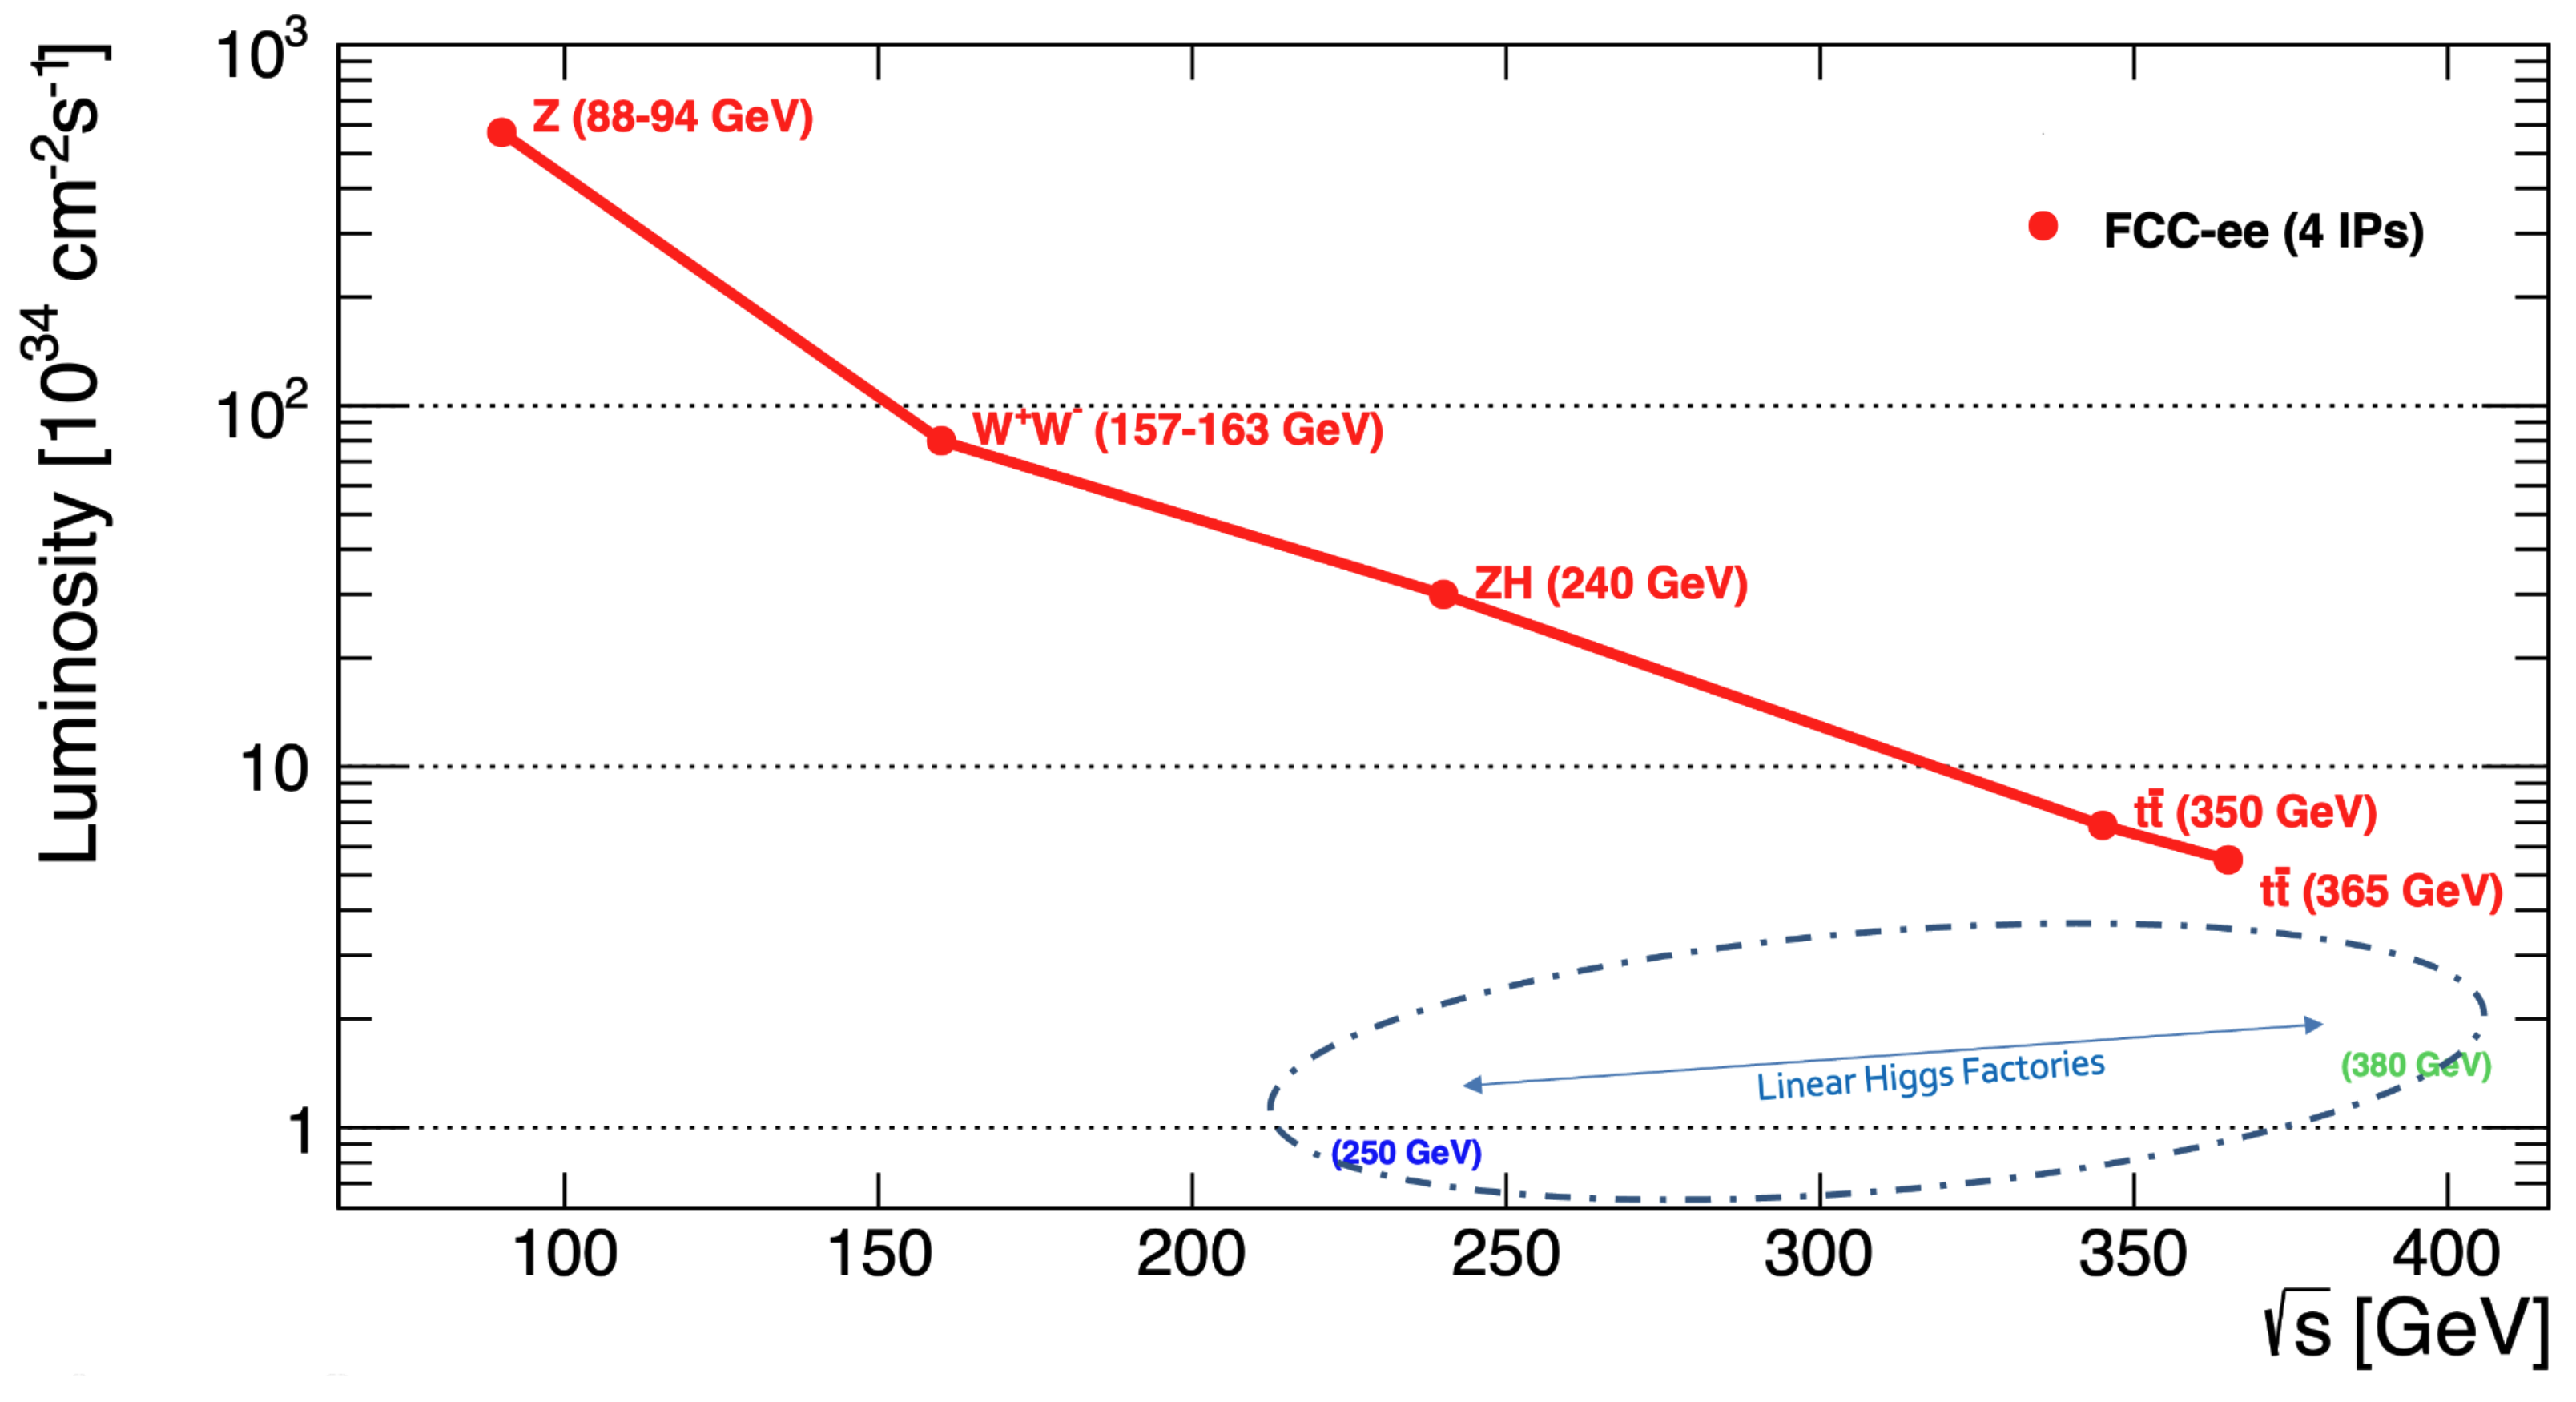
\includegraphics[width=0.77\textwidth]{Overview/Figs/FCCeeLumis2024.png}
\caption{The FCC-ee baseline design luminosity, summed over 4~IPs, displayed as a function of the centre-of-mass energy, 
from the \PZ pole to the $\PQt\PAQt$ threshold and beyond (red curve).
The luminosity typically achievable by linear $\Pep\Pem$ Higgs factories with a single IP in their baseline design between 250 and 380\,GeV is also indicated (dash-dotted oval in the lower-right corner of the figure).}
\label{fig:FCCeeLumis} 
\end{figure}

\begin{table}[ht]
\renewcommand{\arraystretch}{0.95}
\centering
\caption{The baseline FCC-ee operation model with four interaction points, showing the centre-of-mass energies, design instantaneous luminosities for each IP, and integrated luminosity per year summed over 4~IPs.  
The integrated luminosity values correspond to 185 days of physics per year and a 75\% operational efficiency (i.e., $1.2 \times 10^7$ seconds per year)~\cite{Bordry:2645151}, in the \PZ, $\PW\PW$, $\PZ\PH$, and $\PQt\PAQt$ baseline sequence. 
The last two rows indicate the total integrated luminosity and number of events expected to be produced in the four detectors. 
The number of $\PW\PW$ events includes all $\sqrt{s}$ values from 157.5\,GeV up.
\label{tab:seqbaseline}}
\begin{tabular}{lccccccc}
\hline 
Working point & \PZ pole & $\PW\PW$ thresh.\ & $\PZ\PH$ & \multicolumn{2}{c}{$\PQt\PAQt$} \\ \hline
$\sqrt{s}$ {(GeV)} & 88, 91, 94 & 157, 163 & 240 & 340--350 & 365 \\ 
Lumi/IP {($10^{34}$\,cm$^{-2}$s$^{-1}$)} & 140 & 20 & 7.5 & 1.8 & 1.4 \\ 
Lumi/year {(ab$^{-1}$)} & 68 & 9.6 & 3.6 & 0.83 & 0.67 \\ 
Run time {(year)} & 4 & 2 & 3 & 1 & 4 \\ 
Integrated lumi.\ {(ab$^{-1}$)} & 205 & 19.2 & 10.8 & 0.42 & 2.70 \\ \hline
 &  &  & $2.2 \times 10^6$ $\PZ\PH$ & \multicolumn{2}{c}{$2 \times 10^6$ $\PQt\PAQt$} \\
Number of events &  $6 \times 10^{12}$ \PZ & $2.4 \times 10^8$ $\PW\PW$ & $+$ & \multicolumn{2}{c}{$+\,370$k $\PZ\PH$} \\
 &  &  & 65k $\PW\PW \to \PH$ & \multicolumn{2}{c}{$+\,92$k $\PW\PW \to \PH$} \\ \hline
\end{tabular} 
\end{table}

The currently envisioned working hypotheses for the operation model~\cite{janot_2024_nfs96-89q08}, i.e.\ for the overall sequence and the duration of each step, will be continuously optimised in the coming years. 
An example of a baseline sequence is displayed in Fig.~\ref{fig:seqbaseline}, 
with the \PZ, $\PW\PW$, and $\PZ\PH$ runs assumed to happen in this chronological order. 
In reality, however, there will be quasi-total flexibility in the choice of the running sequence. 
(See inset below: `A quasi total flexibility'.) 
This flexibility will accommodate the likely requests of the user community and will also fit the possible need for runs at different energies in view of complementary measurements.

\begin{figure}[ht]
\centering
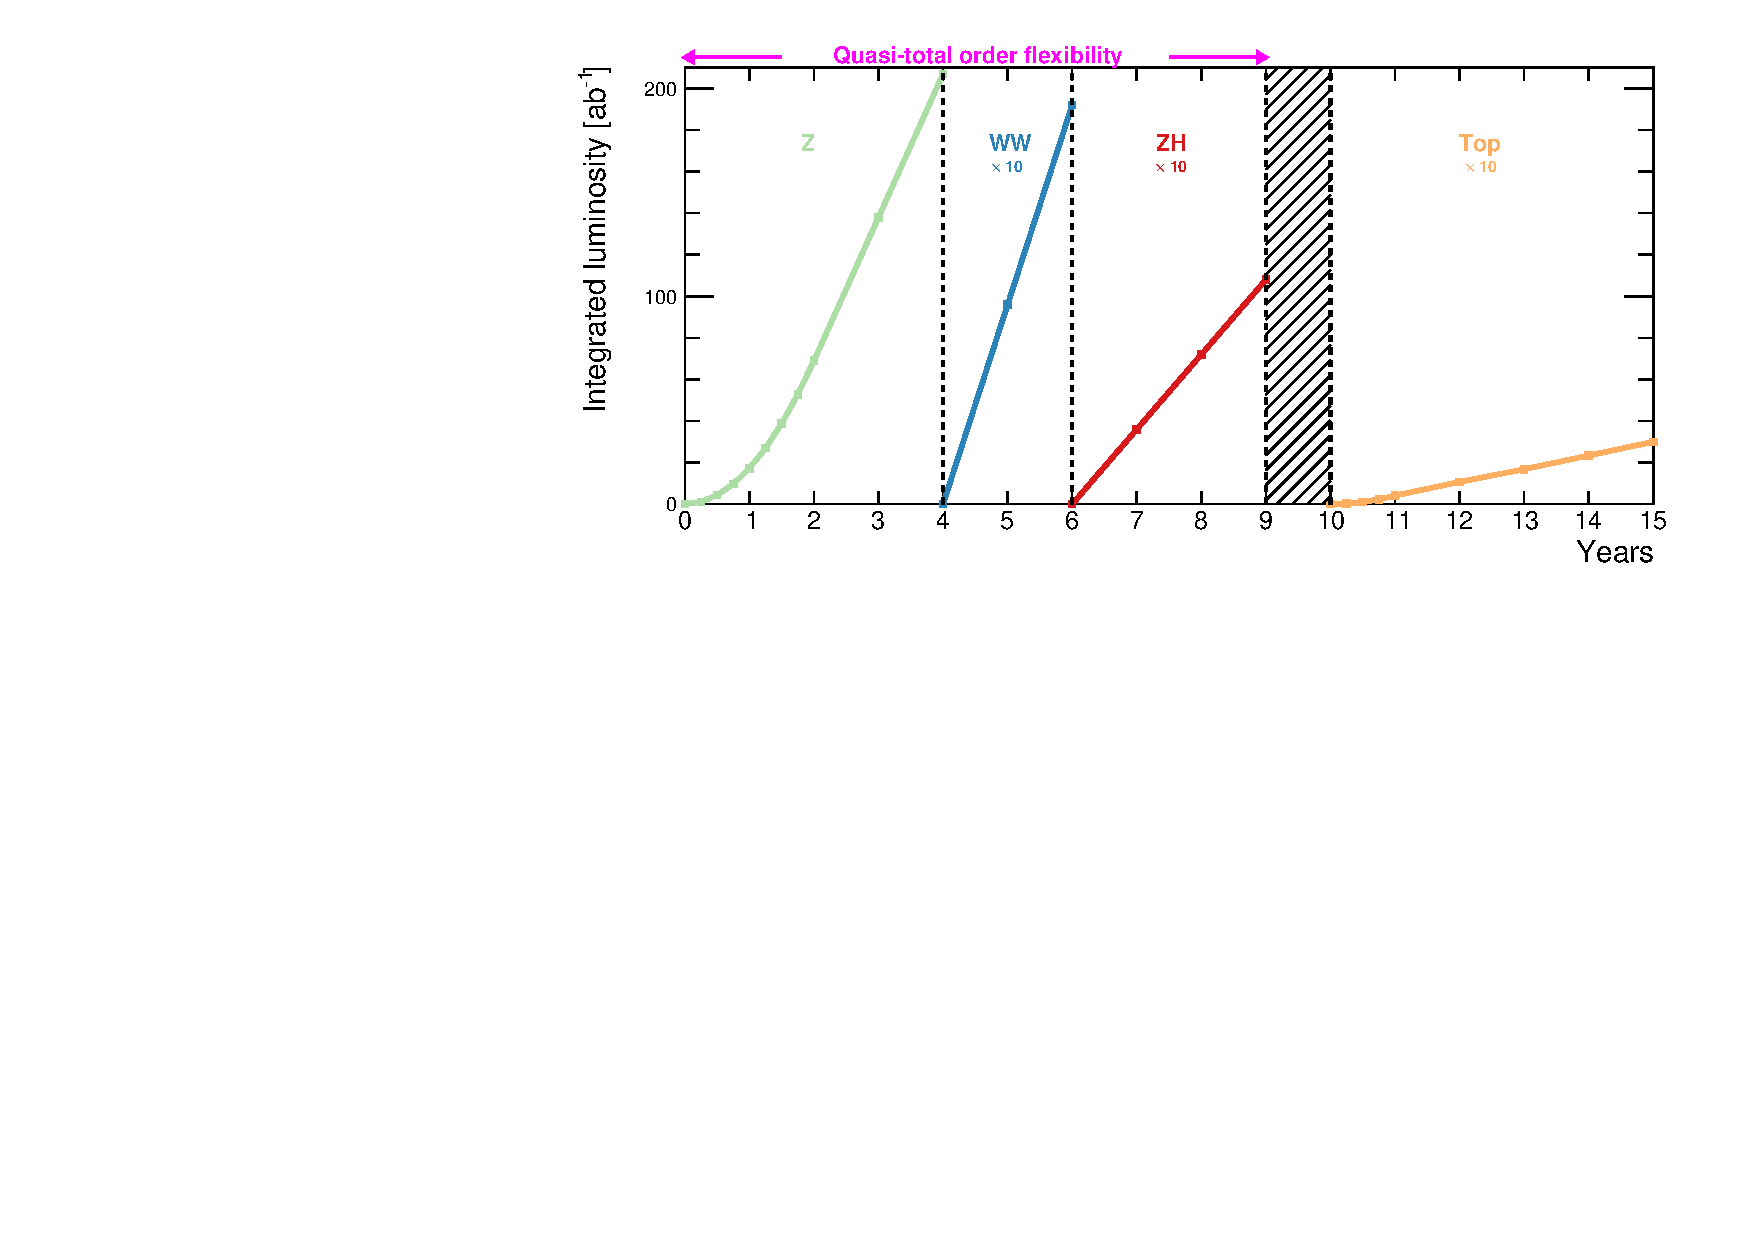
\includegraphics[width=0.85\textwidth]{Overview/Figs/FCCeeSequenceBaseline.pdf}
\caption{\small Baseline operation model for FCC-ee with four interaction points, showing the integrated luminosity at the \PZ pole (green), the $\PW\PW$ threshold (blue), the Higgs factory (red), and the $\PQt\PAQt$ threshold (orange) as a function of time. 
In this baseline model, the sequence of events follows the increase in collision energy, but there is quasi-total flexibility in the sequence all the way to 240\,GeV (see inset). 
The integrated luminosities delivered during the first two years at the \PZ pole and the first year at the $\PQt\PAQt$ threshold are half of the annual design value. 
The hatched area indicates the shutdown time needed to prepare for the higher energy runs at the $\PQt\PAQt$ threshold and beyond.}
\label{fig:seqbaseline} 
\end{figure}

\begin{tcolorbox}[colback=red!5!white,
                  colframe=red!75!black,
                  title=A quasi-total flexibility
                 ]
\footnotesize In Ref.~\cite{note-FCCeeSequence} it was deemed essential to establish the technical and financial feasibility of scheduling a \PZ pole run after the $\PZ\PH$ run or the $\PW\PW$ threshold run, ideally with a first \PZ pole run during the initial period of FCC-ee operation. 
Indeed, the \PZ pole run, while extremely fertile in physics opportunities, is undoubtedly the most ambitious and demanding part of the programme from all perspectives (accelerator, energy calibration, detectors systematic biases, theory calculations).
It will be extremely challenging to achieve all the goals of the \PZ pole run during the first four years of the collider operation. 
\tcblower
\footnotesize This requirement from physics was compounded by a recommendation from the mid-term review committees to 
{\it consolidate (and ideally simplify) the design of the RF system to allow efficient energy-staging, as well as to reduce complexity, risk, and cost; and to study options to avoid the 1-cell/2-cell RF cavity reconfiguration between \PZ and $\PZ\PH$/$\PW\PW$ running, in order to simplify the SRF system implementation and to improve flexibility in the physics programme.} 
The new versatile RF system designed accordingly (see Ref.~\cite{FCC-PED-FSR-Vol2})
enables a quasi-total flexibility to choose the running sequence. 
For example, it would allow for short (few weeks) initial \PZ pole and $\PW\PW$ threshold runs, to commission the collider and the detectors, to establish the resonant depolarisation procedures for centre-of-mass energy calibration, etc. 
The $\PZ\PH$ run could then proceed early, before going back to the \PZ pole and the $\PW\PW$ threshold, both now at full luminosity, with fully functional resonant depolarisation and a complete understanding of the collider.
\end{tcolorbox}

It will ultimately be up to the experimental collaborations and the relevant scientific committees to optimise the time flexibility 
and to tailor the FCC-ee operation scenario according to a number of factors that cannot be mastered today. 
For example, external events such as the FCC-hh magnet readiness or the CERN financial situation may call for a change in the overall duration of the FCC-ee running time. 
Meanwhile, new avenues will be explored during the next phase of the FCC study, between April 2025 and the end of 2027, 
towards increasing the luminosities at all energies, 
as it would be highly beneficial across the whole programme and would make a qualitative difference in a number of cases. 

The original motivation for an $\Pep\Pem$ circular collider was to create a high-luminosity Higgs Factory, operating at $\sqrt{s}=240$\,GeV in the LEP/LHC tunnel~\cite{Blondel:2011fua,Blondel:2012ey,Azzi:2012yn}. 
Choosing to build it in the 80--100\,km tunnel that would ultimately be hosting a 100\,TeV hadron collider was cardinal in making this machine unique on the Higgs factory market. 
To start with, such a tunnel enables a highly versatile Higgs Factory that extends much beyond the study of the Higgs boson alone, for three main reasons:

\begin{enumerate}
\item A circumference of 80--100\,km is required for an $\Pep\Pem$ circular collider to reach (for the first time in $\Pep\Pem$ collisions) the top-pair production threshold, making the FCC-ee energy range optimal to sharpen and challenge our current physics knowledge by studying all SM particles. 
In particular, enabling precise top quark measurements is essential for the overall FCC electroweak and Higgs precision physics programme.

\vspace{0.4cm}

\item For a given power and centre-of-mass energy, the luminosity of a circular collider is roughly proportional to the ring circumference. 
A circumference of 80--100\,km makes FCC-ee the $\Pep\Pem$ electroweak, Higgs, and top factory project with the highest luminosity proposed to date, able to produce, when summing all the data collected at the 4~IPs, $6\times 10^{12}$ \PZ bosons, $2.4\times 10^{8}$ \PW pairs, almost $3\times 10^6$ Higgs bosons, and $2\times 10^6$ top pairs, in as little as 15 years. 
(See also inset below: `Rationale for the operation model').
\end{enumerate}

\begin{tcolorbox}[colback=blue!5!white,
                  colframe=blue!75!black,
                  title=Rationale for the operation model 
                 ]
\footnotesize (From the mid-term review) 
{\it It would also be interesting to add more information in the final Feasibility report about the optimisation of the durations of the various energy runs (\PZ, $\PW\PW$, $\PZ\PH$, $\PQt\PAQt$) as well as a more detailed and quantitative discussion demonstrating the importance of the $\PQt\PAQt$ running.}
\tcblower
\footnotesize The baseline set of centre-of-mass energies and integrated luminosities is found to be the most sensible way to distribute luminosity within the 15 years overall running constraint. 
It is deemed sufficient to establish a minimal, yet remarkable, physics outcome for such a collider, with the smallest possible set of centre-of-mass energies that enables a study of all particles of the SM with a real chance of discovery. 

\begin{itemize}
\item At the \PZ pole ($\sqrt{s} = 91.2$\,GeV), at least $5\times 10^{12}$ \PZ (in two years) enables otherwise unreachable flavour (\PQb, \PQc, $\Pgt$) physics, studies of QCD and hadronisation, the search for rare or forbidden decays, and the exploration of the dark sector. 
Together with the runs at $\sqrt{s} \simeq 88$ and $94$\,GeV, the \PZ pole data yield 50 to 1000-fold improved measurements of the \PZ line-shape and many electroweak precision observables (EWPO), including the \PZ invisible width. 
An integrated luminosity of at least 40\,ab$^{-1} $ at the two energies, just below and just above the \PZ pole (one year each), was deemed appropriate for a direct, unique, and statistically limited determination of $\alpha_\text{QED}(m_{\PZ})$ and $\alpha_\mathrm{S}(m_{\PZ})$, 
which otherwise would greatly limit the new physics interpretation of all measurements of $\sin^2\theta_{\PW}^\text{eff}$. 
One of the findings of the study has been the realisation of how rich the run at and around the \PZ pole is for the FCC-ee physics outcome.
\item An integrated luminosity of at least 20\,ab$^{-1}$ in two years around the $\PW^+\PW^-$ production threshold, evenly shared between $\sqrt{s} = 157.5$ and 162.5\,GeV, is needed for the measurement of the \PW mass (and decay width) with a statistical precision commensurate with the expected precision of the centre-of-mass energy determination. 
These data are also important for, in particular, the determination of the number of neutrino species and for an independent measurement of the strong coupling constant.
\item An integrated luminosity of at least 10\,ab$^{-1}$ in three years at $\sqrt{s} = 240$\,GeV provides model-independent measurements of the Higgs boson couplings from a combination of its  branching fractions and of the total $\PZ\PH$ production cross section. 
In particular, a per-mil precision can be reached on the coupling of the Higgs boson to the \PZ, which greatly constrains new physics coupled to the Higgs boson.  
\item A short run to scan the $\PQt\PAQt$ threshold ($\sqrt{s} = 340$--350\,GeV) allows the measurement of the top-quark mass, a fundamental parameter of the Standard Model, with a precision of $\cal O$(10\,MeV), for which hadron colliders cannot compete. 
Because the prediction of EWPO's is, in various ways, sensitive to $m_\text{top}$, the discovery power of this EWPO exploration is limited by the uncertainty on $m_\text{top}$. 
For example, matching the precision of the SM predictions from the EWPO measurements to the 180\,keV (resp.\ 4\,keV) statistical uncertainty on the \PW mass (resp.\ \PZ width) requires a 20\,MeV (resp.\ 15\,MeV) knowledge of $m_\text{top}$.  
It is only when the mass of the top quark mass is measured with this precision that the FCC-ee EWPO measurements give their best sensitivity, typically increasing the reach in new physics energy scale by 60\%. 
\item 
The $\PZ\PH$ cross section dependence on $\sqrt{s}$ provides sensitivity to the Higgs boson self-coupling when data at 365\,GeV are available, allowing a 5\,$\sigma$ discovery of this coupling to be contemplated. 
More importantly, the per-cent measurement of the top EW couplings 
{\it(i)}~matches the EWPO ppm precision at the \PZ pole and the $\PW\PW$ threshold; 
and {\it (ii)}~keeps the theoretical uncertainties on the top Yukawa coupling determination 
at FCC-hh at the per-cent level, a pre-requisite for the model-independent determination of the Higgs boson self-coupling.
\end{itemize}
\end{tcolorbox}

\begin{itemize}
\item[3.] A circumference of 80--100\,km is also required for FCC-ee to offer unparalleled control of the centre-of-mass energy, not only at the \PZ pole but also at the $\PW\PW$ threshold, with the use of resonant depolarisation~\cite{Blondel:2019jmp,Blondel:2021zix}. 
At the \PZ pole, the centre-of-mass energy scale should be known to 1\,ppm or better, 
with a point-to-point residual uncertainty of 28\,keV and a per-mil level spread. 
These parameters are key inputs to the electroweak precision programme~\cite{Maestre:2021zvq}. 
Details are given in Chapter~\ref{sec:epol}. 
The resulting precisions on the \PZ mass and width, the forward-backward asymmetry of muon pairs around the \PZ pole, the electromagnetic coupling constant $\alpha_\text{QED}(m_{\PZ})$, as well as on the \PW mass, are listed in the first rows of Table~\ref{tab:EWPO}.  
\end{itemize}

\noindent Several other fundamental aspects add to the uniqueness of FCC-ee.

\begin{enumerate}

\item One of the findings of the FCC feasibility study has been the realisation of how rich the intensity-frontier multi-Tera-Z run is for the FCC-ee physics outcome. 
It promises comprehensive measurements of the \PZ lineshape and many EWPOs with at least fifty-fold improved precision, as well as direct and uniquely precise determinations of the
$\alpha_\text{QED}(m_{\PZ})$~\cite{Janot:2015gjr,Riembau:2025ppc} and $\alpha_\mathrm{S}(m_{\PZ})$ interaction couplings (Table~\ref{tab:EWPO}), which would otherwise be dominant parametric uncertainties for virtually all precision SM calculations. 
The comparison of these data with commensurately accurate SM predictions is a way to reveal the existence of new physics (or to severely constrain its properties) through virtual loops or mixing: a factor of 50 in precision corresponds to a factor of 7 in energy scale, representing a step towards discovery 
(Section~\ref{sec:PhysicsCaseBSM} and Refs.~\cite{Allwicher:2024sso,Gargalionis:2024jaw}) 
similar to that from LHC to FCC-hh.  
This \PZ pole run offers more than `just higher precision'. 
It also enables otherwise unreachable flavour (\PQb, \PQc, \Pgt) physics, studies of QCD and hadronisation, the search for rare or forbidden decays, the exploration of the dark sector, and significantly increases sensitivity to new feebly interacting particles, altogether further increasing the prospects for discovery. 

\item A unique feature of circular colliders is the ability to serve several IPs. Another finding of the FCC Feasibility Study has been the demonstration of the importance of operating four detectors (instead of only two in the 2014--2018 Conceptual Design Study), which led to an optimisation of the ring layout with a new four-fold periodicity 
(further increasing the synergies with FCC-hh). 
In a configuration with 4~IPs, the FCC science value for the investment is maximised in multiple ways. 
(See inset below: `The benefits of four interaction points'.) 

\item Finally, FCC-ee stands out among the Higgs Factory projects for its unique opportunity to access the Higgs boson coupling to electrons~\cite{Ghosh:2015gpa,Dery:2017axi,Altmannshofer:2015qra}, through the resonant production process \mbox{$\Pep\Pem \to \PH$} at $\sqrt{s} = 125$\,GeV~\cite{dEnterria:2021xij}. 
This measurement relies on the combination of the high luminosity, the possibility of operating four detectors, the continuous ppm centre-of-mass energy control, and the ability for centre-of-mass monochromatisation~\cite{FausGolfe2021}. 
This is a unique opportunity for FCC-ee, and one of its toughest challenges. 

\end{enumerate}

As a Higgs factory, FCC-ee has all the advantages of an $\Pep\Pem$ collider running in the vicinity of the $\PZ\PH$ cross section maximum: the measurement of this cross section by counting events with an identified \PZ boson 
(and for which the mass recoiling against the \PZ gathers around the Higgs boson mass~\cite{Azzurri:2021nmy}, independently of the Higgs boson properties details) 
provides a precise and model-independent determination of $\kappa_{\PZ}$, the Higgs boson coupling to the \PZ. 
This absolute measurement can then be used as a `standard candle' by all other measurements, including those made at hadron or muon colliders. 
The position of the \PZ recoil mass peak also provides an accurate measurement of the Higgs boson mass from the precise knowledge of the centre-of-mass energy. 
In combination with the measurement of the rate of $\PZ\PH$ events with a $\PH \to \PZ \PZ^\ast$ decay, proportional to $\kappa_{\PZ}^4/\Gamma_{\PH}$, a model-independent determination of the total width $\Gamma_{\PH}$ can be obtained. 
The analysis of the other decays provides a set of model-independent partial width and coupling measurements. 

\begin{table}[p]
\centering
\caption{Experimental (statistical and systematic) precision expected for a selection of measurements accessible at FCC-ee, 
compared with the present world-average precision~\cite{ParticleDataGroup:2024cfk}. 
Some of the FCC-ee experimental systematic uncertainties (4$^\text{th}$ column) are initial estimates from early 2021~\cite{Blondel:2021ema} and others have been improved and consolidated during the Feasibility Study. 
A goal of further studies will be to improve them down to the level of the statistical uncertainties (3$^\text{rd}$ column) with new ideas and innovative methods.
This set of measurements, together with those of the Higgs boson properties, 
achieves indirect sensitivity to new physics up to a scale $\Lambda$ of 100\,TeV 
in an Effective Field Theory (EFT) description with dimension-6 operators (Chapter~\ref{sec:physics}) 
and possibly much higher in specific new physics (non-decoupling) models.  
\label{tab:EWPO}}
\setlength{\tabcolsep}{1.5pt}
\renewcommand{\arraystretch}{0.80}
{\small
\begin{tabular}{lrclccr}
\toprule
Observable  &  & present &          &  FCC-ee  &  FCC-ee  &  Comment and   \\
            & value  &$\pm$& uncertainty  &  {\bf Stat.} &   Syst.\     & leading  uncertainty \\
\midrule
$m_{\PZ}$ (keV)  &  91\,187\,600   & $\pm$ &  2000    & {\bf 4} & 100  & From \PZ line shape scan  \\
$  $  &  & &    &   &  & Beam energy calibration \\
\midrule
$\Gamma_{\PZ}$ (keV)  & 2\,495\,500   & $\pm$ &  2300    & {\bf 4}  &  12  & From \PZ line shape scan  \\
$  $  &  & &    &   &   &  Beam energy calibration  \\
\midrule
$\sin^2{\theta_{\PW}^\text{eff}} ~ (\times 10^6)$  & 231,480   & $\pm$ &  160   & {\bf 1.2}   &  1.2  & 
From $A_\text{FB}^{\PGm\PGm}$ at \PZ peak\\
$  $  &  & &    &   &   &  Beam energy calibration  \\
\midrule
$1/\alpha_\text{QED} (m_{\PZ}^2) ~ (\times 10^3) $  & 128\,952  & $\pm$ &  14   & {\bf 3.9}   &  small  &
From $A_\text{FB}^{\PGm\PGm}$ off peak\\
& & & & {\bf 0.8} & tbc & From $A_\text{FB}^{\PGm\PGm}$ on peak\\
$  $  &  & &    &   &  &  QED\&EW uncert.\ dominate  \\
\midrule
$ R_{\ell}^{\PZ} ~(\times 10^3)$  & 20\,767 & $\pm$ &  25   & {\bf 0.05}   & 0.05   &  Ratio of hadrons to leptons \\
$  $  &  & &  &  &  &    Acceptance for leptons  \\
\midrule
$ \alpha_\mathrm{S} (m_{\PZ}^2) ~(\times 10^4) $  & 1\,196 & $\pm$ &  30  &  {\bf 0.1}  &  1  &
Combined ${R_{\ell}^{\PZ}},\,\Gamma^{\PZ}_\text{tot},\,\sigma^{0}_\text{had}$ fit\\
\midrule
$ \sigma^{0}_\text{had}~(\times 10^3)$ (nb) & 41\,480.2 & $\pm$ &  32.5    & {\bf 0.03}  &  0.8  &  Peak hadronic cross section  \\
$  $  &  & &    &  &   &  Luminosity measurement  \\
\midrule 
$ {N_{\PGn}}  (\times 10^3) $  & 2\,996.3  & $\pm$ &  7.4   & {\bf 0.09}   &  0.12 &  \PZ peak cross sections \\
$  $  &   &  &    &   &  &   Luminosity measurement \\
\midrule
$ R_{\PQb} ~(\times 10^6) $  & 216\,290 & $\pm$ &  660   & {\bf 0.25}    &  0.3  &  Ratio of $\PQb\PAQb$ to hadrons  \\
%$  $  &  & &    &   &  &  Stat.\ extrapol.\ from SLD
%\\
\midrule
$ A_\text{FB}^{\PQb,0} ~(\times 10^4) $  & 992 & $\pm$ &  16   & {\bf 0.04}   &  0.04  &  \PQb-quark asymmetry at \PZ pole  \\
$  $  &  & &  &   &  &    From jet charge \\
\midrule
$ A_\text{FB}^{\text{pol},\Pgt} ~(\times 10^4) $  & 1\,498 & $\pm$ &  49  & {\bf 0.07}   &  0.2  &  \Pgt\ polarisation asymmetry  \\
$  $  &  & &    &   &  &  \Pgt\ decay physics \\
\midrule
\Pgt\ lifetime (fs)  &  290.3  & $\pm$ &  0.5   &  {\bf 0.001}   & 0.005   &  ISR, \Pgt\ mass  \\
\midrule 
\Pgt\ mass (MeV)  & 1\,776.93 & $\pm$ & 0.09  & {\bf 0.002} & 0.02   & estimator bias, ISR, FSR \\
\midrule 
\Pgt\ leptonic ($\PGm \PGnGm \PGnGt$) BR (\%) & 17.38 & $\pm$ & 0.04  & {\bf 0.00007} & 0.003   &  PID, $\pi^0$ efficiency \\ 
\midrule 
$ m_{\PW}$ (MeV)  &  80\,360.2 & $\pm$ &  9.9    & {\bf 0.18}  & 0.16  & From $\PW\PW$ threshold scan \\
$  $  &  & &    &   &  &  Beam energy calibration  \\
\midrule
$\Gamma_{\PW}$ (MeV)  & 2\,085   & $\pm$ &  42    & {\bf 0.27}  & 0.2  & From $\PW\PW$ threshold scan \\
$  $  &  & &    &  &   &  Beam energy calibration  \\
\midrule
$ \alpha_\mathrm{S} (m_{\PW}^2) ~ (\times 10^4)$  & 1\,010   & $\pm$ & 270 &  {\bf 2}  & 2  &
  Combined $R_{\ell}^{\PW},\,\Gamma^{\PW}_\text{tot}$ fit\\
\midrule
$ N_{\PGn} ~ (\times 10^3) $  & 2\,920 & $\pm$ &  50   & {\bf 0.5}   & small   &   Ratio of invis.\ to leptonic \\
$  $  &  & &    &   &  & in radiative \PZ returns  \\
\midrule
$m_\text{top}$ (MeV) &  172\,570 & $\pm$ &  290    & {\bf 4.2}  & 4.9 %35  
& From $\PQt\PAQt$ threshold scan \\
$  $  &  & &    &   & &  QCD uncert.\ dominate \\
\midrule
$\Gamma_\text{top}$ (MeV) &  1\,420   & $\pm$ &  190    &{\bf 10}  & 
6 %25  
& From $\PQt\PAQt$ threshold scan \\
$  $  &  & &    & & &  QCD uncert.\ dominate \\
\midrule
$\lambda_\text{top}/\lambda_\text{top}^\text{SM}$  &   1.2   & $\pm$ &  0.3    & {\bf 0.015} & 
0.015 %0.10  
& From $\PQt\PAQt$ threshold scan \\
$  $  &  & &    &   &  &  QCD uncert.\ dominate \\
\midrule
$\PQt\PQt\PZ$ couplings &
   & $\pm$ &  30\%   & {\bf 0.5--1.5} \%  & small  & From $\sqrt{s}=365$\,GeV run  \\
\bottomrule
\end{tabular}
}
\end{table}

\begin{tcolorbox}[colback=green!5!white,
                  colframe=green!75!black,
                  title=The benefits of four interaction points
                 ]
\footnotesize (From the mid-term review) 
{\it The Scientific Advisory Committee recommends to construct 4~IPs for FCC-ee from the beginning. 
The Scientific Policy Committee finds the proposal to include more than two IPs an attractive option. 
However, we expect, for the final Feasibility report, arguments focusing not only on the na{\"\i}ive luminosity gain but also on the overall physics optimisation.}
\tcblower
\footnotesize

{\bf Detector Diversity}
The diverse set of demanding physics measurements and searches at FCC-ee leads to many different challenging detector requirements, which cannot be simultaneously satisfied by only one or even two detectors. 
Instead, four FCC-ee interaction points allow for a broader diversity of detector solutions to be explored and, therefore, a wider community with diverse interests and skills to join the FCC-ee project, with a better perspective of optimally covering all FCC-ee physics opportunities. 
Detector diversity also allows cross-checks of results across experiments: a single experiment is quite vulnerable to unforeseen effects, and consistency between two experiments can still happen by chance. 
Such bad luck is much less likely with four diverse detectors. 
(See remark about redundancy below.)  

{\bf Improved sustainability} 
Operating FCC-ee with 4~IPs provides a net gain of luminosity (typically up to a factor 1.7 with respect to the 2~IP option) for a given electricity consumption. 
The physics outcome of 15 years operation with 4~IPs would require 25 years with just 2~IPs. 
Running with four experiments would decrease the FCC-ee operation carbon emissions in the same proportions. Folding in the construction carbon budget of the tunnel the additional two IPs and two detectors, it is found that operating FCC-ee with 4~IPs would reduce the total carbon footprint by $\sim$\,15\% for the same physics outcome as with 2~IPs, both with today's figures and with those expected in the construction and operation times of FCC-ee.

{\bf Reduced and more robust systematic uncertainties} 
In order to fully benefit from the considerable FCC-ee event samples, especially at the \PZ pole, most of the work will focus on reducing the systematic uncertainties to match the statistical precision. 
As a matter of fact, many key measurements are potentially affected by detector-related systematic biases. 
These biases are uncorrelated between experiments, so that the related systematic uncertainties scale down as $1/\sqrt{N_\text{experiments}}$. 
Precision is also about redundancy: measuring the same quantity in several experiments can reveal sources of errors that would have been overlooked otherwise. 
The illustrative example closest to FCC-ee comes from the LEP measurement of the \PZ mass with the 1991 data, when a large discrepancy of $\sim 20 \pm 5$\,MeV was noticed between the measurements from L3 and OPAL, on the one hand, and the measurements from ALEPH and DELPHI, on the other. 
The investigation that followed identified and solved the origin of the issue, but it could have remained unnoticed for a long time (or forever) had there been only ALEPH and DELPHI (or only L3 and OPAL) around the ring.

{\bf Collider monitoring} 
With the large collision rate at the \PZ pole, each detector will act as sophisticated beam instrumentation by allowing quick and high-quality measurements of many beam parameters: positions and sizes of the luminous regions; longitudinal and transverse boosts of the collision at the four IPs (beam energy difference, centre-of-mass energy spread, crossing angle); the dependence of these parameters on the exact position of the collision within each bunch; and other information we have not thought of yet. 
These measurements at four different points of the collider provide a huge amount of information on the beam properties, which is useful for collider performance optimisation and, more specifically, on the `energy model', which is the cornerstone of the precision programme at the \PZ pole, at the $\PW\PW$ threshold, and even more so at the Higgs boson resonance ($\sqrt{s} = 125$\,GeV).   

{\bf Time flexibility} 
The additional flexibility offered by two additional interaction points could be a game changer for the FCC-ee scientific outcome. 
For example, reaching the $5\sigma$ discovery level for the Higgs self-coupling, contemplating a first measurement of the electron Yukawa coupling, or securing a thorough search for sterile neutrinos, would simply be missed opportunities with only two IPs (a little over 2\,$\sigma$ significance expected).
The larger luminosity expected with four IPs allows for a different time allocation to the different centre-of-mass energies, to be optimised when the time comes, by the FCC-ee user community.

{\bf Community building} 
The FCC-hh will require the participation of an even larger community of users than the LHC. 
The large collaborations operating the four detectors at FCC-ee would raise the overall profile of the worldwide high-energy frontier community to a level more appropriate to support the ultimate high-energy proton collider.

{\bf Integrated luminosity gain} 
Many FCC-ee measurements are statistically limited, either directly (e.g., the direct determination of $\alpha_{\rm QED}(m_{\rm Z}^2)$ from the muon forward-backward asymmetry measurements at $\sqrt{s}=88$ and 94\,GeV) or because their experimental systematic uncertainties would continue to improve with additional data, as is the case for many critical observables (e.g., the \PZ width, the effective mixing angle, etc.). 
Any increase of integrated luminosity is also welcome for searches for feebly interacting particles or for rare/forbidden processes. 
Therefore, these measurements and searches immediately benefit from four interaction points. 
\end{tcolorbox}

The FCC-ee best-measured Higgs boson couplings, $\kappa_{\PZ}$ and $\kappa_{\PW}$, with a precision of 0.1\% and 0.23\%, after eight years of operation at $\sqrt{s} \geq 240$\,GeV, respectively, would require half a century to be reached with linear $\Pep\Pem$ Higgs factories running either at 250 and 500\,GeV or at 380 and 1500\,GeV, making FCC-ee the most time- and cost-effective, as well as the most sustainable, Higgs factory of all proposed options~\cite{Janot:2022jtn,Blondel:2024mry}. 
More details on the physics programme are given in Chapter~\ref{sec:physics}. 

The many new opportunities of physics measurements and searches at FCC-ee create at least as many challenges. 
Reaching experimental and theoretical systematic uncertainties commensurate with the statistical precision of the many measurements feasible at FCC-ee requires a careful study of the detector concepts, possibly of the mode of operation, and of theoretical developments. 

The FCC-ee physics programme presents a number of key theoretical challenges~\cite{Heinemeyer:2021rgq}. 
Generally speaking, the aim is either to provide the tools to compare experimental observations to theoretical predictions at a level of precision similar or better than the (statistical) experimental uncertainties (Table~\ref{tab:EWPO}), or to identify the additional calculations, tools, observables, or experimental inputs that are required to achieve this level of precision.
Another essential line of research to be followed jointly by theorists and experimenters is to identify observables, or ratios of observables, for which experimental and/or theoretical uncertainties can be reduced. 
Finally, both for motivational purposes and for prioritisation, the relative impact of the various measurements on the search for new physics should be evaluated. The theoretical work motivated by the FCC programme can be organised as follows.

\begin{itemize}
\item  Calculation of QED (mostly), EW, and QCD corrections to (differential) cross sections, needed to convert experimental measurements to so-called `pseudo-observables': couplings, masses, partial widths, asymmetries, etc., without altering significantly the possible new-physics contributions in the original measurements.
Appropriately accurate event generators are essential for the implementation of these effects in the experimental procedures.
\item  Calculation of the pseudo-observables with the precision required in the framework of the Standard Model so as to take full advantage of the experimental precision.
\item 
Identification of the limiting issues, such as the questions related to the definition of parameters, in particular the treatment of quark masses and, more generally, QCD objects.
\item Investigation of the sensitivity of the proposed (or new) experimental observables to the effect of new physics in a number of important, specific scenarios. 
This essential work must be done at an early stage, before the project is fully designed, since it potentially affects the priorities for detector concepts and for the running plan.
\end{itemize}

A community of theorists has already risen to the precision challenges, especially at the \PZ peak~\cite{Blondel:2018mad}. 
An evaluation of the options for the path ahead can be found in Refs.~\cite{Blondel:2019qlh,Freitas:2019bre,Heinemeyer:2021rgq}, and is developed in Chapter~\ref{sec:theory}.

A complete set of detector specifications and their impact on the physics measurements is another main deliverable of the feasibility study. 
The performance of a number of options for the various detector components of possible future detectors: calorimeters~\cite{Aleksa:2021ztd}, tracking and vertex detectors~\cite{Barchetta:2021ibt}, muon detectors~\cite{Braibant:2021wts}, luminometers~\cite{Dam:2021sdj}, and particle identification devices~\cite{Wilkinson:2021ehf} are being studied to understand how they could meet the requirements. 
More details are given in Chapter~\ref{sec:concepts}. 
The following gives a brief idea of the type of requirements that are under study. 

\begin{itemize}
\item {\bf Higgs and top physics}
A set of requirements have been established by past linear collider studies for Higgs and top physics at 240 
and 340--365\,GeV, arising in particular from the desired performance of particle-flow reconstruction, flavour tagging, or lepton momentum measurement. 
They need to be adapted to take into account the cleaner FCC-ee experimental environment, the smaller beam-pipe radius, and the smaller maximum operating energy~\cite{Azzi:2021gwg}. 
Additional requirements arise, related to the need for a more accurate Higgs boson mass determination~\cite{Azzurri:2021nmy} prior to the $s$-channel Higgs boson production run, and for a more accurate $\PZ\PH$ cross section measurement, to enable a determination of the  Higgs self-coupling. 
The $s$-channel Higgs boson production also leads to demanding requirements on the centre-of-mass energy monochromatisation, while keeping a high luminosity and calling for the most sensitive analysis to separate Higgs boson decays from the huge background of $\Pep\Pem$ annihilation events~\cite{dEnterria:2021xij}. 

\item {\bf Tera-Z challenges}
The high luminosity and large event rate at the \PZ pole (over 100\,kHz), to which simulated data need to be added, turn into considerable challenges for data taking, storage and processing. 
The \PZ lineshape determination, which is based on cross section measurements as a function of the centre-of-mass energy for hadronic and leptonic decays of the \PZ, requires accurate mechanical construction and in-situ alignment of the luminometer and detector end-caps, in view of acquiring precise knowledge of the central tracker and calorimeter acceptance, for the dilepton and diphoton events (and, to a lesser extent, for hadronic events). 
The point-to-point centre-of-mass-energy uncertainties of the resonance scan, which can be verified in particular by means of the muon pair mass and boost reconstruction, are most relevant for the \PZ width and the forward-backward asymmetry measurements. 
The accuracy of the mass reconstruction needed sets stringent constraints on the stability of the momentum reconstruction over time and scan points~\cite{Maestre:2021zvq}. 
With a statistical precision of 4\,\keV for both the \PZ mass and the \PZ width, the centre-of-mass determination is critical for the physics output of the Tera-Z run~\cite{Blondel:2019jmp,note_EPOL}.

\item {\bf Physics with \PW pairs} 
The sub-MeV precision on the \PW mass expected from a scan of the $\PW\PW$ production threshold seems, a priori, more demanding on the centre-of-mass energy calibration, and on the theoretical understanding of the cross section, than on the detector itself. 
At higher energies, the requirements on jet angular calibrations and the possible dependence of the precise knowledge of the composition of hadrons in these jets, however, should be revisited. 
Similarly, requirements on lepton angle, energy reconstruction, and energy scale, should be established~\cite{Azzurri:2021yvl}, although they are probably covered by the requirements from the \PZ run.

\item {\bf Flavour challenges}
The formidable progress of the performance of vertexing devices in the past two decades, paired with the five times smaller beam-pipe diameter with respect to LEP, leads to unprecedented \PQb- and \PQc-tagging performance. 
The resulting expected statistical uncertainties on the flavour EWPOs, such as $R_{\PQb,\PQc}$ or $A_\text{FB}^{\PQb,\PQc}$, 
allow for much larger improvements (by up to a factor of 2000) with respect to the LEP measurements of other EWPOs. 
In addition, the rich FCC-ee flavour programme can be fully exploited only if the detector is equipped with hadron identification covering the effective momentum range at the \PZ resonance~\cite{WilkinsonFCCPhys3} and electromagnetic calorimetry with a superb energy resolution~\cite{AleksanFCCPhys4}.

\item {\bf Tau physics}
The $\Pgt$ measurements listed in Table~\ref{tab:EWPO} (lifetime, mass, and branching fractions) have the potential to achieve a determination of the Fermi constant at the level of a few $10^{-5}$. 
These measurements provide some of the most demanding detector requirements on momentum resolution (for the mass resolution), on the knowledge of the vertex detector dimensions (for the tau lifetime), and on $\Pe/\PGm/\pi$ separation over the whole momentum range (for the leptonic branching ratios). 
The \Pgt-based EWPOs, $R_{\Pgt}^{\PZ}$, $A_\text{FB}^\text{pol,\Pgt}$, and $P_{\Pgt}$, as well as the detailed study of the hadronic spectral functions, require fine granularity and high efficiency in the tracker and electromagnetic calorimeter~\cite{Dam:2021ibi}.

\item {\bf Feebly interacting particles} 
The current heavy neutral lepton (HNL) search strategy is based on a rather conservative signal selection, requiring in particular an HNL decay less than 1\,m away from the interaction point. 
With four IPs, the discovery region extends to the physical regions favoured by the see-saw models of neutrino masses.
It would be possible to extend it by detecting HNL decays further away from the IP, e.g., by making use of the large amount of cavern space surrounding the detector~\cite{Chrzaszcz:2020emg}. 
Other feebly interacting particles, decaying into non-pointing or delayed photons, pose a different set of challenges, which could possibly benefit from a high-precision timing detector. 
See Section~\ref{sec:HNL} for details. 
\end{itemize}

Integrating all these (initial) detector requirements will be a considerable challenge, commensurate with the unique set of measurement opportunities and with the discovery potential offered by FCC-ee.  
A refined list of detector requirements is being derived from a number of case studies inspired by the set of physics benchmark measurements at FCC-ee (encompassing those presented in Table~\ref{tab:EWPO}), as described in Refs.~\cite{SnowmassBenchmarkProcesses,Azzi:2021ylt}. 
The four FCC interaction points will not be too many to cover the resulting variety of detector requirements and physics opportunities. 
More details are given in Chapter~\ref{sec:requirements}.

The experimental environment at FCC-ee, where the incoming beams cross typically a few million times before interacting, is gentle and clean compared to hadron colliders, muon colliders and even linear $\Pep\Pem$ colliders. 
The main challenges have been extensively studied by the Machine Detector Interface group~\cite{Boscolo:2019awb}:
\begin{itemize}
    \item The design of the $\Pep$ and $\Pem$ rings is asymmetric around each interaction region, in order to eliminate the need for strong bending magnets upstream of the collision points and thus minimise the synchrotron radiation background in the detectors.
    \item The large number of bunches and the low level of beamstrahlung radiation result in a low rate of pile-up events, typically $2\times 10^{-3}$ at the \PZ pole and less than $10^{-2}$ at the top energies.
    \item The strong focusing optics requires a short free space (2.2\,m) between the last beam elements. 
    A compensating solenoid and quadrupole assembly that fits in a forward dead cone of no more than 100\,mrad, has been designed and a complete mock-up is being prepared.   
    \item The luminosity monitors situated in front of this assembly could be adapted to the geometry with two beam pipes crossing at an angle of 30\,mrad.
    \item The small beam transverse dimensions allow for a beam pipe of 10\,mm radius and for the first layer of the vertex detector to be installed very close to the vacuum chamber.
    \item In the current design with compensating solenoids, the detector solenoid magnetic field must be limited to 2\,T when operating at the \PZ pole, to avoid a blow up of the vertical beam emittance and a resulting loss of luminosity. 
    Alternative designs with non-local compensation are being studied.  
\end{itemize}

These conditions are favourable on several accounts. 
The 100\,mrad low angle dead cone offers the possibility to extend the detector coverage down to a polar angle of $\cos{\theta}\simeq 0.99$, while the 10\,mm radius beam pipe should be a prime starting point for high efficiency \PQb- and \PQc-flavour tagging against light quarks and gluons. 
The 2\,T magnetic field limit is not a significant handicap since the momentum of the produced partons is typically distributed around 50\,GeV and does not exceed 183\,GeV. 
If needed, an increase of the magnetic field to 3\,T or more can be envisioned at higher energies, without loss of luminosity. 
More details about the challenges pertaining to the machine-detector interface and beam backgrounds are given in Chapter~\ref{sec:mdi}.

The work for the particle physicists is now clearly cut out: design the experimental setup and prepare the theoretical tools that can, demonstrably, fully exploit the capabilities of FCC-ee. 
Experimentation at FCC-ee is both relatively easy and extremely demanding. 
The experimental conditions are clean, with essentially no pile-up, a well-defined and controllable centre-of-mass energy, and benign beamstrahlung and synchrotron radiation effects. 
The sophistication arises from the very richness of the programme. 
Matching the experimental and theoretical accuracy to the statistical precision, and the detector configuration to the variety of channels and discovery cases, will be the real challenge.